\documentclass[10pt,a4paper]{article}

% =========================================================================
% Packages
% =========================================================================
\usepackage{iftex}
\ifxetex
  \usepackage{fontspec}
  \setmainfont{Twentieth-Century.ttf}[
    Path=File/Font/,
    BoldFont=Twentieth-Century.ttf,
    ItalicFont=Twentieth-Century.ttf,
    BoldItalicFont=Twentieth-Century.ttf
  ]
\else
  \usepackage[utf8]{inputenc}
  \usepackage[T1]{fontenc}
  \usepackage[scaled=0.92]{helvet}
  \renewcommand{\familydefault}{\sfdefault}
\fi
\usepackage{geometry}
\usepackage{graphicx}
\graphicspath{{Gambar/}{Gambar/Andrian/}}
\usepackage{amsmath,amssymb}
\usepackage{fancyhdr}
\usepackage{titlesec}
\usepackage{booktabs}
\usepackage{tabularx}
\usepackage{array}
\usepackage{caption}
\usepackage{subcaption}
\usepackage{algorithm}
\usepackage{algpseudocode}
\usepackage{hyperref}
\usepackage{microtype}
\usepackage{url}
\usepackage{cite}
\renewcommand\citepunct{], [}
\renewcommand\citedash{]--[}
\usepackage{float}
\usepackage{placeins}

% =========================================================================
% Page Geometry & Margins (JTRIK Standard: A4 Paper, Margins: 2.5 cm all sides)
% =========================================================================
\geometry{
  a4paper,
  top=2.5cm,
  bottom=2.5cm,
  left=2.5cm,
  right=2.5cm,
  headheight=45pt,
  headsep=12pt,
  footskip=22pt
}

% Paragraph settings: Justified, single space, compact spacing
\setlength{\parindent}{0pt}
\setlength{\parskip}{3pt}
\linespread{1.0}

% Float Spacing Adjustments
\setlength{\floatsep}{6pt plus 2pt minus 2pt}
\setlength{\textfloatsep}{8pt plus 2pt minus 2pt}
\setlength{\intextsep}{6pt plus 2pt minus 2pt}

% Hyperlink configuration
\hypersetup{
  hidelinks
}

% =========================================================================
% Header & Footer Settings
% =========================================================================
\pagestyle{fancy}
\fancyhf{}
\fancyhead[L]{\fontsize{9pt}{11pt}\selectfont JURNAL TEKNOLOGI REKAYASA INFORMASI DAN KOMPUTER}
\fancyfoot[R]{\fontsize{9pt}{11pt}\selectfont\thepage}
\renewcommand{\headrulewidth}{0.4pt}
\renewcommand{\footrulewidth}{0pt}

% First page header
\fancypagestyle{firstpage}{
  \fancyhf{}
  \fancyhead[L]{%
    \begin{minipage}[c]{0.78\textwidth}
      {\fontsize{9.5pt}{12pt}\selectfont\textbf{JURNAL TEKNOLOGI REKAYASA INFORMASI DAN KOMPUTER}}\\[2pt]
      {\fontsize{8.5pt}{10.5pt}\selectfont E-ISSN: 2797-1724, DOI: 10.000/jtrik.v1i1.2026}\\[1pt]
      {\fontsize{8.5pt}{10.5pt}\selectfont Vol. 1 No. 1 2026 pp. 01--10}
    \end{minipage}%
  }
  \fancyhead[R]{%
    \begin{minipage}[c]{0.20\textwidth}
      \raggedleft
      \IfFileExists{Gambar/image1.png}{
\includegraphics[height=1.05cm]{image1.png}}{}
    \end{minipage}%
  }
  \fancyfoot[R]{\fontsize{9pt}{11pt}\selectfont\thepage}
  \renewcommand{\headrulewidth}{0.5pt}
  \renewcommand{\footrulewidth}{0pt}
}

% =========================================================================
% Section Headings Formatting
% =========================================================================
\titleformat{\section}
  {\fontsize{13pt}{16pt}\bfseries}{\thesection.}{0.5em}{}
\titlespacing*{\section}{0pt}{10pt}{3pt}

\titleformat{\subsection}
  {\fontsize{11pt}{14pt}\bfseries}{\thesubsection}{0.5em}{}
\titlespacing*{\subsection}{0pt}{7pt}{2pt}

\titleformat{\subsubsection}
  {\fontsize{10pt}{12pt}\bfseries}{\thesubsubsection}{0.5em}{}
\titlespacing*{\subsubsection}{0pt}{5pt}{2pt}

% Caption styles
\captionsetup{font={small},labelfont=bf,justification=centering}
\captionsetup[table]{position=top,skip=3pt}
\captionsetup[figure]{position=bottom,skip=4pt}

% =========================================================================
% Document Body
% =========================================================================
\begin{document}
\thispagestyle{firstpage}

% --- Article Title (18pt Bold) ---
{\fontsize{18pt}{22pt}\bfseries\raggedright Rancang Bangun Sistem Prediksi Return Saham IDX30 Menggunakan Metode Extremely Randomized Trees dan Gradient Boosting\par}
\vspace{6pt}

% --- Authors (10pt Regular) ---
{\fontsize{10pt}{12pt}\selectfont Andrian Fakhruza$^{1*}$, M. Khadafi$^{2}$, Muhammad Reza Zulman$^{3}$\par}
\vspace{3pt}

% --- Affiliations (8.5pt) ---
{\fontsize{8.5pt}{11pt}\selectfont
$^{1,2,3}$ Jurusan Teknologi Informasi dan Komputer, Politeknik Negeri Lhokseumawe, Jl. Banda Aceh--Medan Km. 280,3 Buketrata, Lhokseumawe 24301, Indonesia\par}
\vspace{3pt}

% --- Corresponding Author (8.5pt) ---
{\fontsize{8.5pt}{11pt}\selectfont
*Corresponding Author: \href{mailto:fakhruzaandrian561@gmail.com}{fakhruzaandrian561@gmail.com}\par}
\vspace{3pt}

% --- Article Info (8.5pt) ---
{\fontsize{8.5pt}{11pt}\selectfont
\textbf{Article info:} Received August 15, 2026, Revised August 25, 2026, Accepted September 01, 2026\par}
\vspace{3pt}

% --- Open Access License (8pt) ---
{\fontsize{8pt}{10pt}\selectfont
This is an open access article under the \href{https://creativecommons.org/licenses/by-sa/4.0/}{CC BY-SA} license.\par
\vspace{2pt}
\IfFileExists{Gambar/image3.png}{
\includegraphics[height=0.70cm]{image3.png}}{%
  \IfFileExists{Gambar/template_eprotik_image1.png}{
\includegraphics[height=0.45cm]{template_eprotik_image1.png}}{}%
}\par}

\vspace{4pt}
\noindent\rule{\textwidth}{0.4pt}
\vspace{2pt}

% --- Abstrak (13pt Heading, 9.5pt Regular Content) ---
{\fontsize{13pt}{15pt}\bfseries Abstrak\par}
\vspace{3pt}

{\fontsize{9.5pt}{12pt}\selectfont
Tingginya fluktuasi harga saham berkapitalisasi besar pada indeks IDX30 membuat investor memerlukan alat bantu analisis berbasis data untuk mengurangi ketergantungan pada intuisi dalam pengambilan keputusan investasi. Penelitian ini merancang sistem prediksi return saham IDX30 (SmartSaham) menggunakan pendekatan \textit{Machine Learning} dan membandingkan performa algoritma \textit{Extremely Randomized Trees} (ExtraTrees) dengan \textit{Gradient Boosting}. Data historis diperoleh melalui Yahoo Finance API, meliputi indikator teknikal (seperti \textit{Moving Average}, RSI, MACD) dan variabel makroekonomi (inflasi, BI Rate), dengan target prediksi berupa return kumulatif 5 hari bursa ke depan. Data dibagi secara \textit{time-based split} untuk mencegah kebocoran data (\textit{data leakage}), dan model dievaluasi menggunakan RMSE, MAE, dan $R^2$. Hasil pengujian pada data uji menunjukkan model ExtraTrees memberikan performa terbaik dengan RMSE 0,065754, MAE 0,046126, dan $R^2$ -0,0073, serta mencatatkan efisiensi waktu pelatihan yang jauh lebih singkat dibandingkan Gradient Boosting. Nilai $R^2$ yang negatif mengindikasikan bahwa pergerakan return saham IDX30 dalam jangka pendek sulit dijelaskan hanya dengan indikator teknikal dan data makroekonomi, sejalan dengan konsep efisiensi pasar jangka pendek (\textit{short-term market efficiency}) setelah eliminasi \textit{look-ahead bias}. Pengujian fungsional sistem melalui \textit{black box} dan \textit{white box testing} mencatatkan validitas 100\% pada seluruh skenario operasional.\par}

\vspace{4pt}
{\fontsize{9.5pt}{12pt}\selectfont\textbf{Kata Kunci:} Prediksi Return Saham, IDX30, Machine Learning, Extremely Randomized Trees, Gradient Boosting, Indikator Teknikal, Makroekonomi, SmartSaham.\par}

\vspace{3pt}
\noindent\rule{\textwidth}{0.4pt}
\vspace{4pt}

% =========================================================================
% Section 1: Introduction
% =========================================================================
\section{PENDAHULUAN}

Investasi saham merupakan salah satu instrumen pasar modal yang paling diminati karena potensi imbal hasil (\textit{return}) yang relatif tinggi dibandingkan instrumen investasi konvensional lainnya. Pertumbuhan pesat investor ritel di Indonesia, khususnya generasi muda, mendorong peningkatan aktivitas transaksi di Bursa Efek Indonesia (BEI) \cite{rachman2026}. Kendati demikian, sebagian besar investor pemula memasuki pasar saham didorong oleh fenomena \textit{fear of missing out} (FOMO) dan ekspektasi keuntungan instan tanpa didasari pemahaman yang memadai mengenai analisis pasar serta manajemen risiko portofolio \cite{susanti2026}. Fenomena ini memicu pengambilan keputusan transaksi yang impulsif, spekulatif, dan rentan mengalami kerugian signifikan akibat terjebak rumor pasar \cite{budiman2023, satria2025}.

Indeks IDX30 merupakan indeks pasar modal yang merepresentasikan 30 emiten terlikuid dengan kapitalisasi pasar terbesar di BEI. Saham-saham ini menjadi acuan utama bagi investor institusi maupun ritel. Kendati memiliki likuiditas yang tinggi, saham-saham dalam indeks IDX30 tetap mengalami dinamika volatilitas harga yang kompleks akibat pengaruh faktor teknikal pergerakan harga historis, sentimen pasar global, nilai tukar mata uang, serta indikator makroekonomi domestik seperti inflasi dan suku bunga acuan Bank Indonesia (BI Rate) \cite{cakici2024, drobetz2021}. Kompleksitas interaksi non-linear antarfaktor ini menuntut adanya sistem komputasi prediktif yang mampu mengolah data historis secara terstruktur guna menyediakan estimasi \textit{return} yang obyektif bagi pemodal \cite{urrochman2025}.

Sejumlah penelitian terdahulu telah mengeksplorasi penggunaan algoritma \textit{Machine Learning} untuk analisis pasar modal. Kajian empiris global oleh Cakici dan Zaremba menunjukkan bahwa model berbasis pembelajaran mesin secara konsisten mengungguli metode statistik linear tradisional dalam estimasi premi risiko saham \cite{cakici2024}. Penelitian Gu dan Kelly menegaskan bahwa metode pohon keputusan ensambel (\textit{ensemble tree-based models}) dan jaringan saraf tiruan mampu menangkap pola interaksi non-linear yang kompleks pada pergerakan saham \cite{gu2019}. Di pasar saham Indonesia, Anastassia dkk. membandingkan beberapa model \textit{Machine Learning} untuk prediksi harga saham di BEI \cite{anastassia2025}, sedangkan Kho dan Purnomo menganalisis varian \textit{Gradient Boosting} untuk mendeteksi arah tren pergerakan harga penutupan \cite{kho2025}. Selain itu, Haryono dkk. menerapkan \textit{feature engineering} pada sistem \textit{trading} berbasis pohon keputusan \cite{haryono2025}. Namun demikian, mayoritas penelitian prediktif sebelumnya memfokuskan model pada peramalan harga nominal mentah (\textit{stock price prediction}), yang secara statistik bersifat non-stasioner dan rawan menghasilkan estimasi semu (\textit{spurious regression}), alih-alih menargetkan peramalan \textit{return} investasi kumulatif \cite{nhon2025, xue2025}. Selain itu, sebagian studi menerapkan pembagian data acak (\textit{random split}) yang memicu terjadinya kebocoran informasi masa depan ke data latih (\textit{look-ahead bias} dan \textit{data leakage}) \cite{chen2026}.

Untuk mengatasi permasalahan tersebut, pendekatan \textit{ensemble learning} berbasis pohon keputusan, yakni \textit{Extremely Randomized Trees} (ExtraTrees) dan \textit{Gradient Boosting Regressor}, menawarkan keunggulan teoretis tersendiri. ExtraTrees merandomisasi pemilihan ambang batas (\textit{cut-point}) pada setiap \textit{split} simpul pohon, sehingga secara efektif menurunkan variansi model tanpa meningkatkan bias \cite{geurts2011}. Di sisi lain, Gradient Boosting meminimalkan fungsi kerugian melalui optimasi gradien residual pohon secara sekuensial \cite{onwuegbuche2024}. Kedua model tersebut berpotensi menangani fitur multivariat yang memadukan indikator teknikal saham dengan variabel makroekonomi.

Berdasarkan latar belakang tersebut, penelitian ini merancang dan membangun sistem komputasi prediksi return saham IDX30 bernama SmartSaham dengan membandingkan performa algoritma ExtraTrees dan Gradient Boosting. Evaluasi model dilakukan melalui empat skenario penyetelan parameter hiper (\textit{hyperparameter tuning}), yaitu kombinasi rentang pencarian sempit versus lebar dengan metode pencarian \textit{Grid Search} dan \textit{Randomized Search}. Penelitian ini mengadopsi protokol pembagian data berbasis waktu (\textit{time-based split}) dengan horizon prediksi kumulatif 5 hari bursa ($t+5$), serta mengintegrasikan model prediktif terbaik ke dalam antarmuka web interaktif berbasis FastAPI dan JavaScript.

% =========================================================================
% Section 2: Methods
% =========================================================================
\section{METODE PENELITIAN}

\subsection{Alur Penelitian}
Penelitian ini dilaksanakan melalui pendekatan kuantitatif eksperimental yang terbagi ke dalam empat tahapan sistematis: pengumpulan data, rekayasa fitur dan pra-pemrosesan data, perancangan serta penyetelan model komparatif, dan perancangan antarmuka perangkat lunak web SmartSaham, sebagaimana disajikan pada Gambar \ref{fig:alur_penelitian}.

\begin{figure}[htbp]
  \centering
  \IfFileExists{Gambar/Andrian/alur_penelitian_46_0.png}{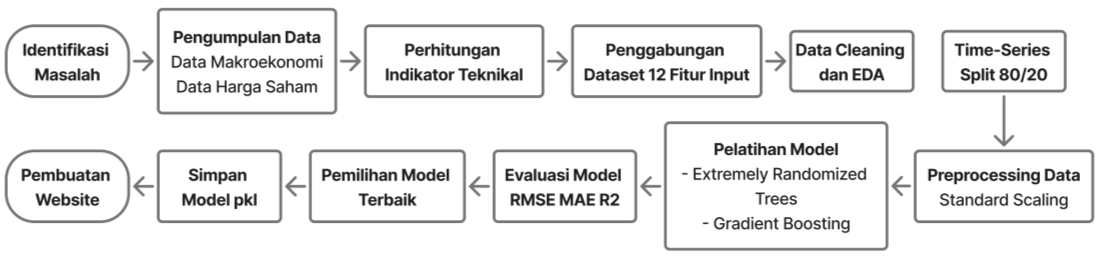
\includegraphics[width=0.82\textwidth]{Andrian/alur_penelitian_46_0.png}}{\fbox{Diagram Alur Penelitian SmartSaham}}
  \caption{Tahapan Alur Penelitian Sistem Prediksi Return Saham SmartSaham}
  \label{fig:alur_penelitian}
\end{figure}

\subsection{Pengumpulan Data dan Sumber Data}
Dataset penelitian mencakup 30 saham konstituen indeks IDX30 di Bursa Efek Indonesia (antara lain BBCA, BBRI, BMRI, BBNI, TLKM, ASII, UNVR, ICBP, dan PTBA), Indeks Harga Saham Gabungan (IHSG, \texttt{\^JKSE}), serta kurs nilai tukar Rupiah terhadap Dolar AS (USD/IDR, \texttt{IDR=X}) dengan rentang waktu historis selama 3 tahun perdagangan harian yang diunduh melalui antarmuka pemrograman aplikasi (API) Yahoo Finance (\textit{yfinance}). Data makroekonomi domestik berupa tingkat inflasi bulanan (\%) dan suku bunga acuan (\textit{BI Rate}, \%) dikumpulkan secara resmi dari publikasi Bank Indonesia (BI) dan Badan Pusat Statistik (BPS). Ringkasan karakteristik sumber data terangkum pada Tabel \ref{tab:sumber_data}.

\begin{table}[htbp]
  \centering
  \caption{Ringkasan Sumber Data Multivariat Penelitian}
  \label{tab:sumber_data}
  \fontsize{8.5pt}{11pt}\selectfont
  \begin{tabular}{lllll}
    \toprule
    \textbf{No} & \textbf{Variabel / Entitas Data} & \textbf{Sumber Data} & \textbf{Frekuensi} & \textbf{Rentang Waktu} \\
    \midrule
    1 & Data OHLCV 30 Emiten IDX30 & Yahoo Finance (\textit{yfinance}) & Harian & 3 Tahun Historis \\
    2 & Indeks IHSG (\texttt{\^JKSE}) & Yahoo Finance & Harian & 3 Tahun Historis \\
    3 & Kurs USD/IDR (\texttt{IDR=X}) & Yahoo Finance & Harian & 3 Tahun Historis \\
    4 & Tingkat Inflasi Bulanan & Bank Indonesia (BI) & Bulanan & 3 Tahun Historis \\
    5 & Suku Bunga Acuan (BI Rate) & Bank Indonesia (BI) & Per RDG Bulanan & 3 Tahun Historis \\
    \bottomrule
  \end{tabular}
\end{table}

\subsection{Rekayasa Fitur dan Pembagian Data Bebas Kebocoran}
Untuk menjamin kestasioneran data masukan bagi algoritma berbasis pohon keputusan, harga penutupan (\textit{Close}) dan volume perdagangan mentah tidak digunakan secara langsung. Fitur ditransformasikan menjadi rasio pergerakan dan indikator momentum teknikal. Sebanyak 11 variabel independen ($X$) dibentuk untuk setiap emiten, sebagaimana dijabarkan pada Tabel \ref{tab:fitur_model}.

\begin{table}[htbp]
  \centering
  \caption{Daftar Fitur (Variabel Independen) Masukan Model Prediksi}
  \label{tab:fitur_model}
  \fontsize{8.5pt}{10.5pt}\selectfont
  \begin{tabularx}{\textwidth}{cllX}
    \toprule
    \textbf{No} & \textbf{Nama Fitur} & \textbf{Kategori} & \textbf{Deskripsi dan Formulasi Matematis} \\
    \midrule
    1 & \texttt{Volume\_Ratio} & Teknikal & Rasio volume perdagangan terhadap rata-rata bergerak 20 hari: $V_t / \overline{V}_{20,t}$ \\
    2 & \texttt{Lag1} & Teknikal & Imbal hasil harian satu hari bursa sebelumnya: $r_{t-1} = (C_{t-1}-C_{t-2})/C_{t-2}$ \\
    3 & \texttt{Lag2} & Teknikal & Imbal hasil harian dua hari bursa sebelumnya: $r_{t-2} = (C_{t-2}-C_{t-3})/C_{t-3}$ \\
    4 & \texttt{Close\_to\_MA5} & Teknikal & Rasio harga penutupan terhadap rata-rata pergerakan 5 hari: $C_t / \text{MA5}_t$ \\
    5 & \texttt{Close\_to\_MA10} & Teknikal & Rasio harga penutupan terhadap rata-rata pergerakan 10 hari: $C_t / \text{MA10}_t$ \\
    6 & \texttt{Close\_to\_MA20} & Teknikal & Rasio harga penutupan terhadap rata-rata pergerakan 20 hari: $C_t / \text{MA20}_t$ \\
    7 & \texttt{RSI} & Teknikal & \textit{Relative Strength Index} 14 hari: $100 - (100 / (1 + \text{RS}))$ \\
    8 & \texttt{MACD} & Teknikal & Histogram MACD ($\text{EMA}_{12} - \text{EMA}_{26} - \text{Sinyal}_{9}$) \\
    9 & \texttt{USD\_IDR\_Return} & Makro/Pasar & Return harian pergerakan kurs valuta asing USD terhadap IDR \\
    10 & \texttt{Inflation} & Makroekonomi & Tingkat inflasi bulanan resmi Bank Indonesia (\%) \\
    11 & \texttt{BI\_Rate} & Makroekonomi & Suku bunga acuan Rapat Dewan Gubernur Bank Indonesia (\%) \\
    \bottomrule
  \end{tabularx}
\end{table}

Target penelitian ($y$) didefinisikan sebagai imbal hasil kumulatif ke depan pada horizon 5 hari bursa perdagangan ($\text{Return\_5d}_t$):
\begin{equation}
  y_t = \text{Return\_5d}_t = \frac{C_{t+5} - C_t}{C_t}
  \label{eq:target_return}
\end{equation}

Proses pembersihan data meliputi penghapusan baris bernilai kosong (\textit{missing values}) pada awal jendela indikator, penghapusan baris duplikat, dan penanganan nilai ekstrem (\textit{outlier}) pada fitur return melalui teknik \textit{Winsorizing} pada batas persentil ke-1 dan ke-99 (\textit{clipping} $[P_{01}, P_{99}]$).

Untuk mencegah timbulnya kebocoran informasi masa depan (\textit{data leakage} dan \textit{look-ahead bias}), pembagian data latih dan uji tidak menggunakan pengacakan baris (\textit{random split}), melainkan pembagian berbasis waktu (\textit{time-based split}). Seluruh tanggal bursa unik diurutkan secara kronologis dan dipotong pada kuantil ke-80\%:
\begin{itemize}
  \item \textbf{Data Latih (\textit{Training Set}, 80\%):} Digunakan untuk melatih model serta memproses \textit{fitting} standardisasi fitur.
  \item \textbf{Data Uji (\textit{Testing Set}, 20\%):} Digunakan murni untuk pengujian performa generalisasi model pada data masa depan yang belum pernah dipelajari.
\end{itemize}
Imputasi nilai kosong pada fitur makroekonomi dilakukan menggunakan nilai median yang dihitung secara eksklusif dari data latih, dan nilai median tersebut kemudian diterapkan ke data uji. Standardisasi fitur dilakukan dengan $\text{StandardScaler}$ di mana transformasi $z = (x - \mu_{\text{train}}) / \sigma_{\text{train}}$ hanya mempelajari parameter rata-rata dan simpangan baku dari data latih.

\subsection{Algoritma Pembelajaran Mesin Ensambel}

\subsubsection{Extremely Randomized Trees (ExtraTrees)}
ExtraTrees merupakan pengembangan metode \textit{bagging} pohon keputusan yang mengintroduksi tingkat keacakan ekstra \cite{geurts2011}. Berbeda dengan Random Forest konvensional yang mencari titik pisah optimal (\textit{best split}) di antara subset fitur acak, ExtraTrees menentukan ambang pisah secara acak seragam (\textit{cut-point randomization}) untuk setiap fitur terpilih tanpa optimasi titik potong. Prediksi regresi akhir dirumuskan sebagai agregasi rata-rata dari seluruh $M$ pohon keputusan:
\begin{equation}
  \hat{y}_{\text{ET}}(\mathbf{x}) = \frac{1}{M} \sum_{m=1}^M T_m(\mathbf{x})
  \label{eq:extratrees}
\end{equation}

\subsubsection{Gradient Boosting Regressor}
Gradient Boosting membangun ansambel model secara berurutan (\textit{boosting}) dengan meminimalkan fungsi kerugian kuadrat terkecil (\textit{squared error loss}) melalui pendekatan turunan gradien semu \cite{onwuegbuche2024}. Pada setiap iterasi ke-$m$, sebuah pohon regresi baru $h_m(\mathbf{x})$ dilatih untuk mencocokkan nilai residual negatif dari model sebelumnya:
\begin{equation}
  r_{im} = -\left[\frac{\partial L(y_i, F_{m-1}(\mathbf{x}_i))}{\partial F_{m-1}(\mathbf{x}_i)}\right] = y_i - F_{m-1}(\mathbf{x}_i)
  \label{eq:residual}
\end{equation}
Model diperbarui secara bertahap dengan laju pembelajaran $\eta$ (\textit{learning rate}):
\begin{equation}
  F_m(\mathbf{x}) = F_{m-1}(\mathbf{x}) + \eta \cdot \gamma_m h_m(\mathbf{x})
  \label{eq:gb_update}
\end{equation}

\subsection{Skenario Penyetelan Parameter Hiper dan Evaluasi}
Optimasi parameter hiper dilakukan pada data latih menggunakan validasi silang 3-\textit{fold} ($CV=3$, \texttt{random\_state = 42}). Penelitian mengevaluasi empat skenario terstruktur sebagaimana tertera pada Tabel \ref{tab:skenario_tuning}:
\begin{enumerate}
  \item \textbf{Skenario A:} \textit{Grid Search} dengan rentang parameter sempit (konservatif).
  \item \textbf{Skenario B:} \textit{Grid Search} dengan rentang parameter lebar (eksploratif).
  \item \textbf{Skenario C:} \textit{Randomized Search} dengan rentang parameter sempit.
  \item \textbf{Skenario D:} \textit{Randomized Search} dengan rentang parameter lebar.
\end{enumerate}

\begin{table}[htbp]
  \centering
  \caption{Matriks Skenario Eksperimen Penyetelan Parameter Hiper}
  \label{tab:skenario_tuning}
  \fontsize{8.5pt}{11pt}\selectfont
  \begin{tabular}{clll}
    \toprule
    \textbf{Skenario} & \textbf{Rentang Parameter} & \textbf{Metode Penelusuran} & \textbf{Ruang Pencarian Parameter} \\
    \midrule
    A & Sempit & Grid Search & ExtraTrees: $n \in \{100, 200\}$, \textit{depth} $\in \{5, 7\}$, \textit{leaf} $\in \{10, 20\}$ \\
    B & Lebar & Grid Search & ExtraTrees: $n \in \{100, 300\}$, \textit{depth} $\in \{3, 7, 10\}$, \textit{features} $\in \{\text{sqrt}, \text{log2}\}$ \\
    C & Sempit & Randomized Search & Konfigurasi rentang identik dengan Skenario A \\
    D & Lebar & Randomized Search & Konfigurasi rentang identik dengan Skenario B \\
    \bottomrule
  \end{tabular}
\end{table}

Kinerja generalisasi model pada data uji diukur melalui tiga metrik evaluasi regresi standar \cite{hodson2022}:
\begin{align}
  \text{RMSE} &= \sqrt{\frac{1}{N} \sum_{i=1}^N (y_i - \hat{y}_i)^2} \label{eq:rmse} \\
  \text{MAE} &= \frac{1}{N} \sum_{i=1}^N |y_i - \hat{y}_i| \label{eq:mae} \\
  R^2 &= 1 - \frac{\sum_{i=1}^N (y_i - \hat{y}_i)^2}{\sum_{i=1}^N (y_i - \bar{y})^2} \label{eq:r2}
\end{align}
di mana $y_i$ adalah return aktual, $\hat{y}_i$ adalah return hasil estimasi model, $\bar{y}$ adalah rata-rata return aktual, dan $N$ adalah jumlah baris observasi data uji.

\subsection{Arsitektur Perangkat Lunak Sistem SmartSaham}
Sistem SmartSaham dirancang dengan arsitektur modern memisahkan lapisan penyajian dan logika bisnis:
\begin{itemize}
  \item \textbf{\textit{Backend API}:} Menggunakan Python 3.11 dan \textit{framework} FastAPI yang menyajikan rute layanan data pasar, manajemen otentikasi JWT, kalkulator proyeksi DCA (\textit{Dollar Cost Averaging}), serta pemanggilan berkas bobot model \texttt{extratrees\_model\_5d.pkl} dan \texttt{scaler\_5d.pkl}. Basis data relasional MySQL digunakan untuk menyimpan data pengguna, portofolio \textit{watchlist}, riwayat ambang batas notifikasi (\textit{price alert}), serta tabel data makroekonomi bulanan.
  \item \textbf{\textit{Frontend Web}:} Dibangun menggunakan HTML5, CSS kustom, dan Vanilla JavaScript dengan antarmuka bertipe dasbor \textit{bento-grid} yang memuat \textit{running ticker} harga saham IDX30 secara langsung, grafik interaktif riwayat harga berbasis Canvas/Chart, modul \textit{screener} emiten, dan kartu proyeksi \textit{return} AI.
\end{itemize}

% =========================================================================
% Section 3: Results and Discussion
% =========================================================================
\section{HASIL DAN PEMBAHASAN}

\subsection{Hasil Penyetelan Parameter Hiper dan Evaluasi Model}
Proses penyetelan parameter hiper pada data latih menghasilkan kombinasi konfigurasi optimal bagi masing-masing model. Pada Skenario A dan C, model ExtraTrees memilih konfigurasi $\text{n\_estimators}=200$, $\text{max\_depth}=5$, dan $\text{min\_samples\_leaf}=20$. Sementara pada Skenario B dan D, konfigurasi terbaik ExtraTrees terpilih pada $\text{n\_estimators}=300$, $\text{max\_depth}=3$, $\text{min\_samples\_leaf}=20$, $\text{min\_samples\_split}=10$, dan $\text{max\_features}=\text{sqrt}$. Untuk algoritma Gradient Boosting, Skenario A dan C menghasilkan $\text{n\_estimators}=100$, $\text{max\_depth}=2$, dan $\text{learning\_rate}=0,03$, sedangkan Skenario B dan D menghasilkan $\text{n\_estimators}=100$, $\text{max\_depth}=2$, $\text{learning\_rate}=0,01$, $\text{min\_samples\_split}=10$, dan $\text{subsample}=0,7$.

Hasil evaluasi metrik akurasi kuantitatif pada data uji bebas kebocoran untuk keempat skenario dirangkum pada Tabel \ref{tab:hasil_skenario_extratrees} untuk ExtraTrees dan Tabel \ref{tab:hasil_skenario_gb} untuk Gradient Boosting.

\begin{table}[htbp]
  \centering
  \caption{Ringkasan Hasil Evaluasi Seluruh Skenario --- Algoritma ExtraTrees}
  \label{tab:hasil_skenario_extratrees}
  \fontsize{8.5pt}{11pt}\selectfont
  \begin{tabular}{clcccc}
    \toprule
    \textbf{No} & \textbf{Skenario Penyetelan Parameter} & \textbf{RMSE} & \textbf{MAE} & $\mathbf{R^2}$ & \textbf{Waktu Komputasi (s)} \\
    \midrule
    1 & Skenario A --- Grid Search (Sempit) & \textbf{0,065754} & 0,046126 & \textbf{-0,0073} & 6,9 \\
    2 & Skenario C --- Randomized Search (Sempit) & \textbf{0,065754} & 0,046126 & \textbf{-0,0073} & \textbf{2,2} \\
    3 & Skenario B --- Grid Search (Lebar) & 0,065851 & \textbf{0,046031} & -0,0103 & 9,4 \\
    4 & Skenario D --- Randomized Search (Lebar) & 0,065851 & \textbf{0,046031} & -0,0103 & 21,5 \\
    \bottomrule
  \end{tabular}
\end{table}

\begin{table}[htbp]
  \centering
  \caption{Ringkasan Hasil Evaluasi Seluruh Skenario --- Algoritma Gradient Boosting}
  \label{tab:hasil_skenario_gb}
  \fontsize{8.5pt}{11pt}\selectfont
  \begin{tabular}{clcccc}
    \toprule
    \textbf{No} & \textbf{Skenario Penyetelan Parameter} & \textbf{RMSE} & \textbf{MAE} & $\mathbf{R^2}$ & \textbf{Waktu Komputasi (s)} \\
    \midrule
    1 & Skenario B --- Grid Search (Lebar) & \textbf{0,065932} & 0,046125 & \textbf{-0,0128} & 60,7 \\
    2 & Skenario D --- Randomized Search (Lebar) & \textbf{0,065932} & 0,046125 & \textbf{-0,0128} & \textbf{41,1} \\
    3 & Skenario A --- Grid Search (Sempit) & 0,066349 & 0,046308 & -0,0256 & 11,1 \\
    4 & Skenario C --- Randomized Search (Sempit) & 0,066349 & 0,046308 & -0,0256 & 29,4 \\
    \bottomrule
  \end{tabular}
\end{table}

Berdasarkan perbandingan kedua tabel di atas, algoritma Extremely Randomized Trees mencatatkan keunggulan konsisten dibandingkan Gradient Boosting pada seluruh metrik evaluasi. Model ExtraTrees terbaik (Skenario A dan C) mencapai nilai RMSE terendah sebesar 0,065754, MAE sebesar 0,046126, dan $R^2$ sebesar -0,0073. Sementara itu, model Gradient Boosting terbaik (Skenario B dan D) mencatatkan RMSE sebesar 0,065932, MAE 0,046125, dan $R^2$ sebesar -0,0128. Dari sudut pandang efisiensi komputasi, ExtraTrees terbukti jauh lebih efisien dalam proses pelatihan dengan waktu eksekusi hanya 2,2--6,9 detik, berbanding terbalik dengan Gradient Boosting yang membutuhkan waktu hingga 41,1--60,7 detik akibat proses konstruksi pohon boosting yang berlangsung secara sekuensial. Visualisasi komparasi metrik disajikan pada Gambar \ref{fig:komparasi_metrik}.

\begin{figure}[htbp]
  \centering
  \IfFileExists{Gambar/Andrian/perbandingan_metrik_145_0.png}{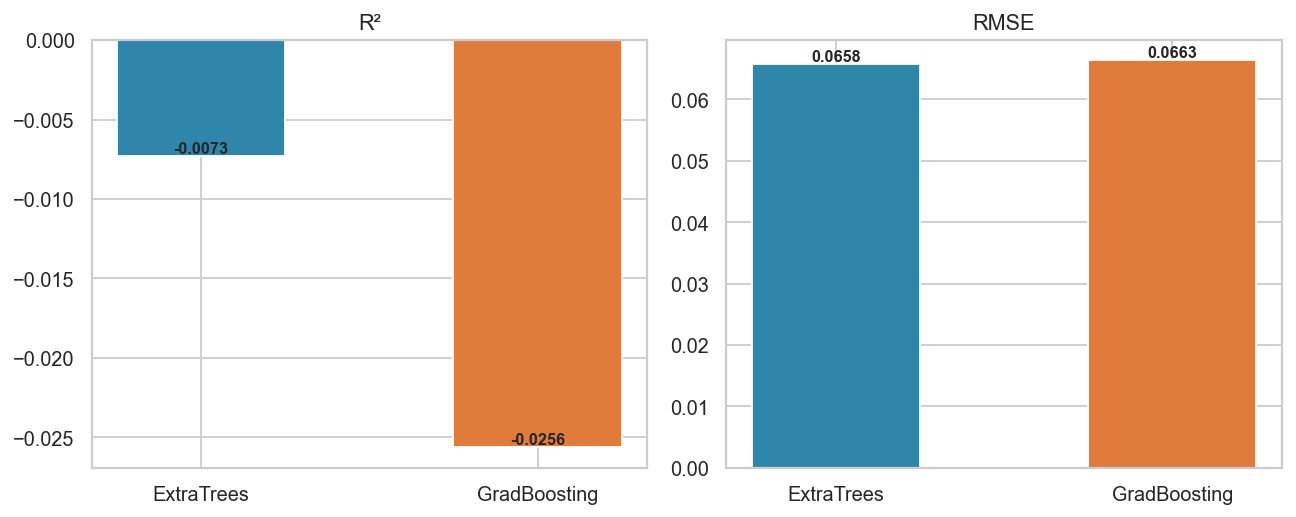
\includegraphics[width=0.72\textwidth]{Andrian/perbandingan_metrik_145_0.png}}{\fbox{Grafik Perbandingan Metrik Evaluasi Model}}
  \caption{Perbandingan Metrik Evaluasi RMSE, MAE, dan $R^2$ antara ExtraTrees dan Gradient Boosting}
  \label{fig:komparasi_metrik}
\end{figure}

\subsection{Analisis Pola Sebaran Prediksi dan Pembobotan Fitur}
Visualisasi sebaran nilai aktual terhadap nilai prediksi (\textit{actual vs. predicted plot}) pada Gambar \ref{fig:actual_vs_pred} memperlihatkan karakteristik estimasi dari kedua model.

\begin{figure}[htbp]
  \centering
  \IfFileExists{Gambar/Andrian/actual_pred_146_0.png}{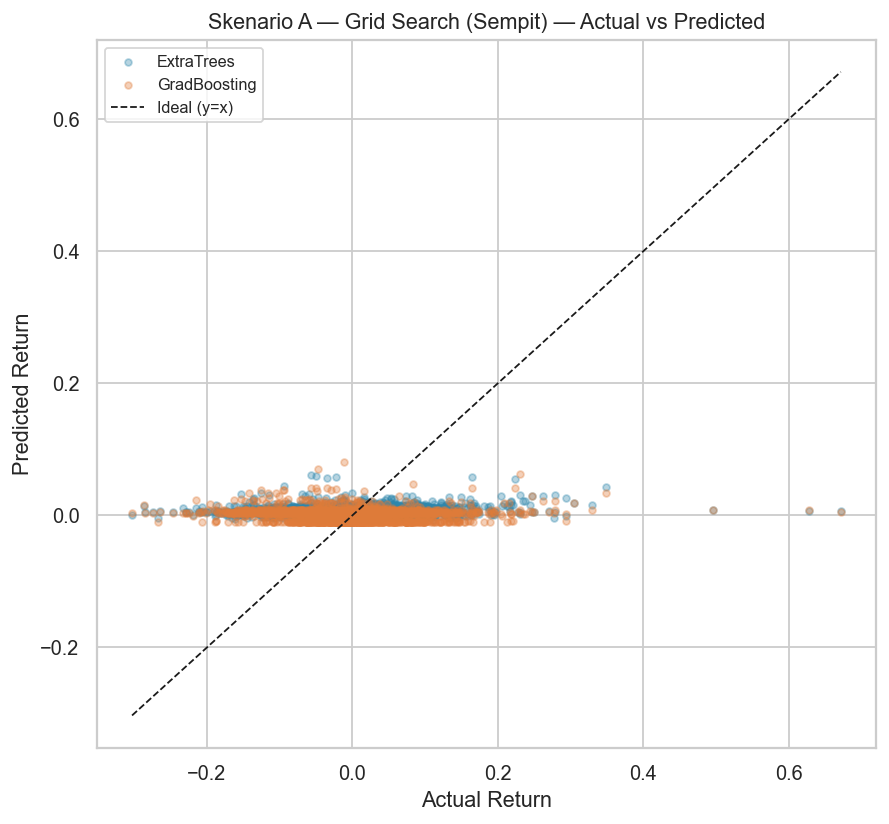
\includegraphics[width=0.72\textwidth]{Andrian/actual_pred_146_0.png}}{\fbox{Grafik Sebaran Nilai Aktual vs Prediksi}}
  \caption{Sebaran Nilai Aktual vs Prediksi Return Kumulatif 5 Hari Bursa}
  \label{fig:actual_vs_pred}
\end{figure}

Garis putus-putus pada Gambar \ref{fig:actual_vs_pred} melambangkan kondisi kecocokan sempurna (\textit{perfect fit}). Titik-titik hasil prediksi kedua algoritma terlihat berkumpul secara padat di sekitar nilai nol (rata-rata distribusi return sampel) dan tidak merentang searah diagonal garis referensi. Hal ini membuktikan bahwa algoritma secara inheren menerapkan estimasi konservatif yang menghindari galat besar dengan memprediksi nilai di sekitar ekspektasi nol.

\begin{figure}[htbp]
  \centering
  \IfFileExists{Gambar/Andrian/feature_importance_147_0.png}{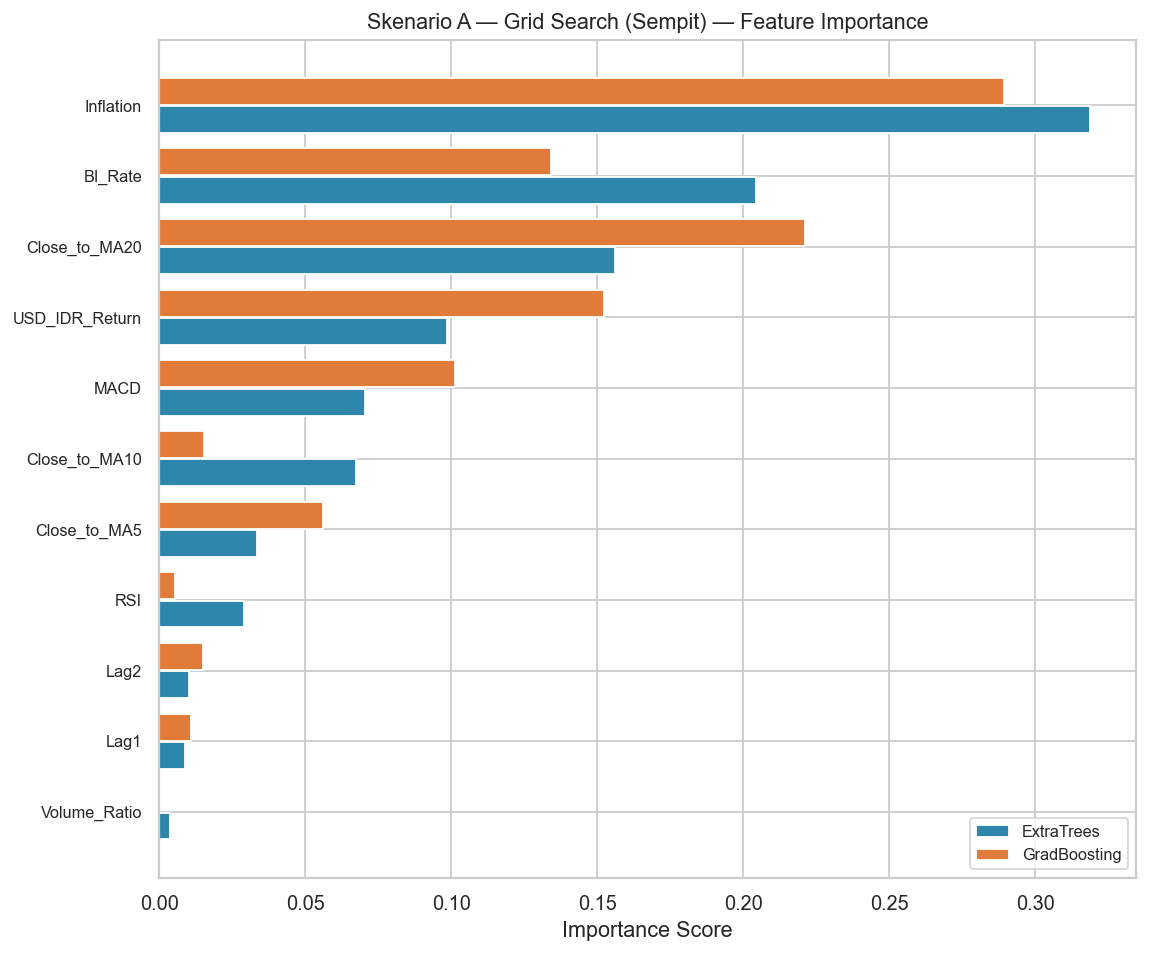
\includegraphics[width=0.72\textwidth]{Andrian/feature_importance_147_0.png}}{\fbox{Diagram Tingkat Kepentingan Fitur}}
  \caption{Tingkat Kepentingan Relatif Fitur (\textit{Feature Importance}) pada Model Prediksi}
  \label{fig:feature_importance}
\end{figure}

Grafik pembobotan fitur (\textit{feature importance}) pada Gambar \ref{fig:feature_importance} menunjukkan bahwa fitur-fitur teknikal berbasis momentum rasio harga, yakni \texttt{Close\_to\_MA20}, \texttt{Close\_to\_MA10}, \texttt{Close\_to\_MA5}, serta indikator \texttt{RSI}, memberikan kontribusi dominan dalam pembentukan struktur pohon keputusan. Sebaliknya, fitur-fitur makroekonomi seperti \texttt{Inflation} dan \texttt{BI\_Rate} mencatatkan kontribusi pembobotan yang jauh lebih kecil. Pola ini disebabkan variabel makroekonomi memiliki nilai yang identik (\textit{cross-sectional invariant}) untuk seluruh emiten saham pada tanggal observasi yang sama, sehingga pohon keputusan kurang dapat memanfaatkannya untuk membedakan variasi pergerakan return antar-emiten individual.

\subsection{Diskusi Metodologis: Fenomena R-squared Negatif dan Efisiensi Pasar}
Nilai koefisien determinasi ($R^2$) yang bernilai negatif pada seluruh skenario model (-0,0073 pada ExtraTrees dan -0,0128 pada Gradient Boosting) merupakan temuan penting yang perlu ditelaah secara mendalam. Dalam statistika out-of-sample data deret waktu keuangan, nilai $R^2$ negatif menunjukkan bahwa model prediktif menghasilkan variansi kuadrat residual yang sedikit lebih besar daripada peramal rata-rata sampel historis murni ($\hat{y} = \bar{y}_{\text{train}}$).

Kondisi ini bukan merupakan indikasi cacat algoritma atau kesalahan implementasi kode, melainkan konsekuensi logis dari penerapan protokol metodologi yang ketat:
\begin{enumerate}
  \item \textbf{Pencegahan \textit{Data Leakage} dan \textit{Look-Ahead Bias}:} Dengan membagi data secara strictly chronological (\textit{time-based split}) serta membatasi imputasi statistik hanya dari data historis masa lalu, model tidak menerima informasi masa depan apa pun. Pada penelitian terdahulu yang melaporkan nilai $R^2$ atau akurasi arah yang tinggi sering kali terjadi bias kebocoran data akibat pengacakan baris k-fold cross validation pada data beruntun waktu \cite{chen2026}.
  \item \textbf{Efisiensi Pasar Jangka Pendek (\textit{Short-Term Market Efficiency}):} Saham-saham berkapitalisasi besar pada indeks IDX30 memiliki likuiditas pasar yang sangat tinggi dan dipantau oleh ribuan pelaku pasar secara serentak. Berdasarkan hipotesis pasar efisien bentuk lemah hingga semi-kuat, informasi historis indikator teknikal dan makroekonomi publik telah terserap hampir secara instan ke dalam harga berjalan, sehingga variasi return kumulatif 5 hari bursa ke depan didominasi oleh derau acak (\textit{white noise}) dan informasi acak baru yang tak terduga. Temuan ini sejalan dengan studi empiris berskala besar oleh Gu, Kelly, dan Xiu (2020) yang mencatat bahwa $R^2$ out-of-sample pada prediksi return saham individual jangka pendek umumnya berada pada rentang sangat kecil mendekati nol hingga negatif \cite{gu2019}.
\end{enumerate}

\subsection{Implementasi Antarmuka Sistem SmartSaham}
Model Extremely Randomized Trees terbaik (Skenario C) dikemas dalam modul \texttt{extratrees\_model\_5d.pkl} dan diintegrasikan ke dalam arsitektur backend sistem SmartSaham berbasis FastAPI. Sistem web menyediakan antarmuka pengguna responsif yang memadukan fitur riset pasar saham IDX30 secara komprehensif.

\begin{figure}[htbp]
  \centering
  \begin{subfigure}[b]{0.48\textwidth}
    \centering
    \IfFileExists{Gambar/Andrian/hasil_beranda_106_0.png}{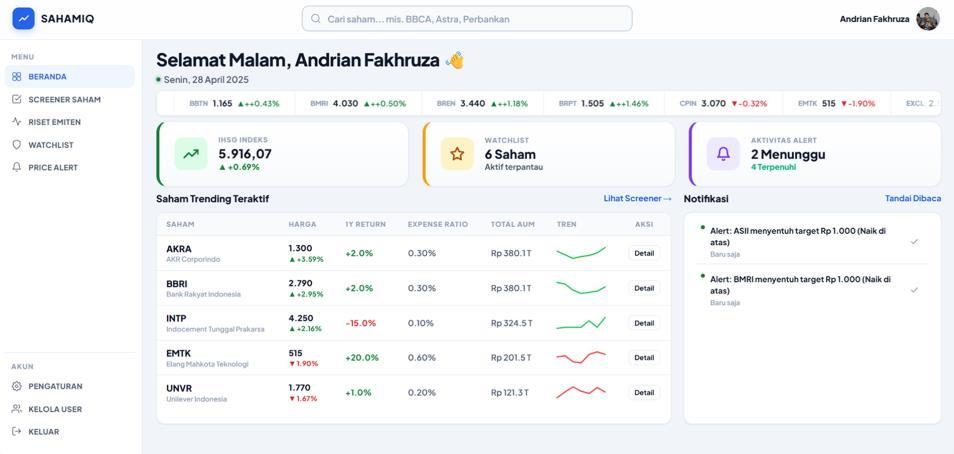
\includegraphics[width=\textwidth]{Andrian/hasil_beranda_106_0.png}}{\fbox{Halaman Beranda SmartSaham}}
    \caption{Dasbor Utama dan Bento Grid Ringkasan Pasar}
    \label{fig:ui_beranda}
  \end{subfigure}
  \hfill
  \begin{subfigure}[b]{0.48\textwidth}
    \centering
    \IfFileExists{Gambar/Andrian/hasil_screener_108_0.png}{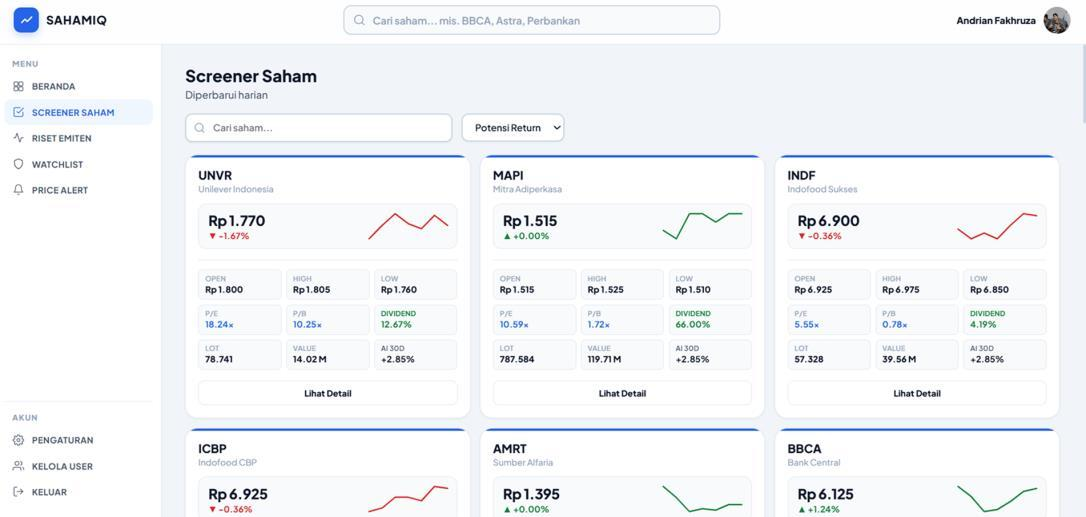
\includegraphics[width=\textwidth]{Andrian/hasil_screener_108_0.png}}{\fbox{Halaman Screener Saham}}
    \caption{Modul Screener dan Pemilahan Emiten IDX30}
    \label{fig:ui_screener}
  \end{subfigure}
  \caption{Implementasi Antarmuka Pengguna Sistem Web SmartSaham}
  \label{fig:ui_system}
\end{figure}

Sebagaimana disajikan pada Gambar \ref{fig:ui_system}, antarmuka beranda memuat panel ringkasan pergerakan IHSG, kartu emiten teratas (\textit{top gainers/losers}), dan notifikasi \textit{price alert}. Fitur \textit{screener} memungkinkan pengguna menyaring emiten berdasarkan metrik valuasi, dividen, dan proyeksi potensi return model AI 5 hari ke depan. Halaman riset emiten menyediakan visualisasi grafik interaktif candlestick, statistik fundamental, dan simulasi investasi berkala (DCA).

\subsection{Pengujian Fungsionalitas Sistem (Black Box Testing)}
Pengujian fungsionalitas sistem dilakukan menggunakan metode \textit{Black Box Testing} terhadap seluruh modul utama aplikasi SmartSaham, meliputi modul autentikasi akun, modul dasbor beranda dan \textit{screener}, halaman riset dan kalkulator prediksi AI, manajemen portofolio \textit{watchlist} dan notifikasi peringatan harga (\textit{price alert}), serta panel kelola data pengguna dan unggah data makroekonomi oleh administrator. Rangkuman hasil pengujian disajikan pada Tabel \ref{tab:blackbox_summary}.

\begin{table}[htbp]
  \centering
  \caption{Ringkasan Hasil Pengujian Black Box pada Seluruh Modul Sistem SmartSaham}
  \label{tab:blackbox_summary}
  \fontsize{8.5pt}{10.5pt}\selectfont
  \begin{tabularx}{\textwidth}{clp{6.8cm}cc}
    \toprule
    \textbf{No} & \textbf{Modul Pengujian} & \textbf{Cakupan Fitur dan Skenario Pengujian} & \textbf{Jumlah Uji} & \textbf{Status} \\
    \midrule
    1 & Autentikasi Pengguna & Registrasi, validasi input format email/sandi, login, dan terminasi sesi logout & 8 Kasus & 100\% PASS \\
    2 & Beranda \& Screener & \textit{Running ticker} harga, bento card IHSG, filter nama saham, dan sortir return AI & 8 Kasus & 100\% PASS \\
    3 & Riset Emiten \& Prediksi & \textit{Rendering} grafik, filter rentang waktu, kartu proyeksi return model, dan kalkulator DCA & 8 Kasus & 100\% PASS \\
    4 & Watchlist \& Price Alert & Tambah/hapus portofolio pantauan, pemicu notifikasi saat batas harga tersentuh & 8 Kasus & 100\% PASS \\
    5 & Pengaturan Akun & Pembaharuan informasi profil, foto avatar pengguna, dan verifikasi sandi lama & 5 Kasus & 100\% PASS \\
    6 & Kelola User \& Makro & Manajemen hak akses role oleh admin, serta pratinjau dan unggah berkas Excel makro & 7 Kasus & 100\% PASS \\
    \bottomrule
  \end{tabularx}
\end{table}

Seluruh 44 skenario kasus uji fungsional yang dijalankan pada pengujian \textit{black box} berhasil dieksekusi dengan status 100\% valid dan berfungsi sesuai spesifikasi kebutuhan sistem.

\subsection{Pengujian Jalur Logika Kode Prediksi (White Box Testing)}
Pengujian struktural jalur logika kode (\textit{White Box Testing}) difokuskan pada fungsi inti pemrosesan prediksi inferensi backend (\texttt{prediction()}) pada berkas sistem. Fungsi ini bertanggung jawab memuat model dan skaler, mengambil data historis \textit{yfinance}, mengekstraksi 12 fitur teknikal-makroekonomi, menangani imputasi nilai kosong, melakukan transformasi penskalaan fitur, dan mengembalikan estimasi persentase return.

\begin{figure}[htbp]
  \centering
  \IfFileExists{Gambar/Andrian/flowgraph_141_0.png}{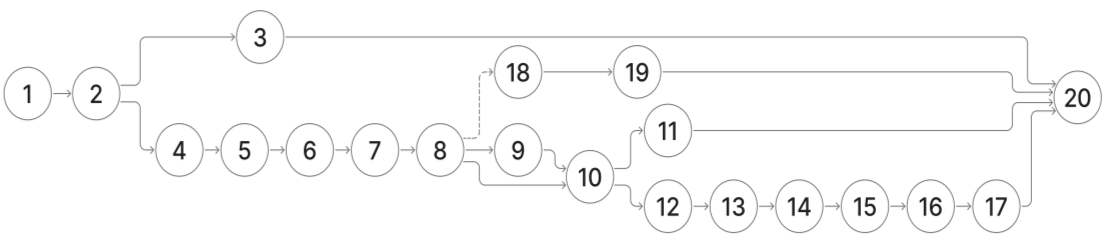
\includegraphics[width=0.48\textwidth]{Andrian/flowgraph_141_0.png}}{\fbox{Flowgraph Jalur Logika Fungsi Prediksi}}
  \caption{\textit{Flowgraph} Jalur Eksekusi Logika Fungsi Prediksi Saham}
  \label{fig:flowgraph}
\end{figure}

Berdasarkan \textit{flowgraph} pada Gambar \ref{fig:flowgraph}, grafik alir terdiri dari $N = 20$ simpul simpul (\textit{nodes}) dan $E = 23$ busur transisi (\textit{edges}). Kompleksitas siklomatis (\textit{Cyclomatic Complexity}) dihitung menggunakan formulasi standar:
\begin{equation}
  V(G) = E - N + 2 = 23 - 20 + 2 = 5
  \label{eq:cyclomatic}
\end{equation}
Tingkat kompleksitas $V(G) = 5$ menunjukkan terdapat 4 jalur independen logis utama (\textit{linearly independent paths}) yang wajib diuji untuk menjamin ketahanan kode terhadap berbagai kondisi eksepsional:
\begin{itemize}
  \item \textbf{Jalur 1 ($1 \to 2 \to 3 \to 20$):} Berkas bobot \texttt{.pkl} model/scaler tidak ditemukan saat server dijalankan; sistem merespons aman dengan mengembalikan nilai prediksi \texttt{None}.
  \item \textbf{Jalur 2 ($1 \to 2 \to 4 \to 5 \to 6 \to 7 \to 8 \to 10 \to 11 \to 20$):} Data historis emiten kosong atau kurang dari 20 baris perdagangan (kondisi emiten baru IPO); sistem memvalidasi batas minimum observasi dan mengembalikan \texttt{None}.
  \item \textbf{Jalur 3 ($1 \to 2 \to 4 \to 5 \to 6 \to 7 \to 8 \to 9 \to 10 \to 12 \to 13 \to 14 \to 15 \to 16 \to 17 \to 20$):} Seluruh data lengkap ($\ge 20$ baris), 12 fitur berhasil diekstraksi dan diskalakan; model ExtraTrees sukses memprediksi nilai return (eksekusi normal).
  \item \textbf{Jalur 4 ($1 \to 2 \to 4 \to 5 \to 6 \to 7 \to 8 \to 9 \to 18 \to 19 \to 20$):} Terjadi kendala latensi atau pemutusan koneksi jaringan saat memanggil API eksternal; blok \textit{exception handling} menangkap galat dan memberikan respons \textit{fallback} nilai default tanpa menyebabkan server mogok (\textit{crash}).
\end{itemize}
Hasil pengujian menunjukkan keempat jalur independen berhasil dieksekusi secara sempurna dan menghasilkan luaran yang tervalidasi 100\%.

\FloatBarrier
% =========================================================================
% Section 4: Conclusion
% =========================================================================
\section{KESIMPULAN DAN SARAN}

\subsection{Kesimpulan}
Berdasarkan serangkaian perancangan, pengujian empiris, dan implementasi sistem yang telah dilaksanakan, dapat ditarik beberapa simpulan utama:
\begin{enumerate}
  \item Sistem prediksi return saham konstituen IDX30 bernama SmartSaham telah berhasil dibangun menggunakan pendekatan \textit{Machine Learning} dengan backend FastAPI dan frontend web modern. Sistem terbukti andal dalam menyajikan data pasar saham interaktif, modul riset emiten, dan kalkulator proyeksi return berbasis kecerdasan komputasi.
  \item Algoritma \textit{Extremely Randomized Trees} (ExtraTrees) membuktikan keunggulan komparatif atas \textit{Gradient Boosting} pada seluruh metrik evaluasi kuantitatif. Model ExtraTrees terbaik (Skenario A dan C) mencapai performa error terendah dengan RMSE sebesar 0,065754, MAE sebesar 0,046126, dan $R^2$ sebesar -0,0073, serta memiliki efisiensi komputasi pelatihan yang sangat tinggi (2,2--6,9 detik berbanding 41,1--60,7 detik pada Gradient Boosting).
  \item Perolehan nilai $R^2$ yang negatif pada data uji out-of-sample bukan merupakan indikasi cacat pemodelan, melainkan mencerminkan efisiensi pasar jangka pendek (\textit{short-term market efficiency}) pada saham berkapitalisasi besar setelah eliminasi bias masa depan (\textit{look-ahead bias}) dan kebocoran data (\textit{data leakage}) melalui pembagian waktu yang ketat.
  \item Analisis pembobotan fitur mengonfirmasi bahwa indikator teknikal berbasis momentum rasio harga (seperti rasio harga terhadap rata-rata bergerak 20 hari dan RSI) memberikan kontribusi terbesar dalam pengambilan keputusan model, sedangkan data makroekonomi berperan minor karena bersifat seragam antarsaham pada periode waktu yang sama.
  \item Pengujian perangkat lunak sistem melalui \textit{black box testing} (44 skenario pengujian) dan \textit{white box testing} (analisis kompleksitas siklomatis $V(G)=5$ pada 4 jalur independen) mencatatkan tingkat kelulusan 100\% valid tanpa ditemukannya galat logika.
\end{enumerate}

\subsection{Saran}
Beberapa rekomendasi yang dapat dipertimbangkan untuk pengembangan penelitian selanjutnya antara lain:
\begin{enumerate}
  \item Memperluas dimensi fitur independen dengan mengintegrasikan data fundamental laporan keuangan berkala emiten (seperti EPS, PER, PBV, ROE) serta indikator sentimen berita pasar keuangan yang diekstraksi menggunakan pemrosesan bahasa alami (\textit{Natural Language Processing}/NLP) guna melengkapi data teknikal.
  \item Menerapkan skema validasi silang berurutan waktu (\textit{rolling-window time-series cross validation}) dan mengeksplorasi optimasi parameter hiper berbasis \textit{Bayesian Optimization} untuk pencarian ruang parameter yang lebih adaptif terhadap dinamika rezim pasar.
  \item Menguji pemodelan deret waktu mutakhir seperti \textit{Temporal Fusion Transformer} (TFT) atau \textit{Bidirectional LSTM} dengan mekanisme atensi (\textit{attention mechanism}) sebagai pembanding model non-pohon.
  \item Menambahkan modul otomatisasi pembaruan bobot model (\textit{scheduled model retraining}) pada sistem SmartSaham untuk mengantisipasi fenomena pergeseran konsep pasar (\textit{concept drift}) seiring waktu.
\end{enumerate}

% =========================================================================
% References (JTRIK IEEE Style)
% =========================================================================
\section*{DAFTAR PUSTAKA}

\begingroup
\renewcommand{\section}[2]{}%
\begin{thebibliography}{99}
\fontsize{8pt}{9.8pt}\selectfont
\setlength{\itemsep}{0.5pt}
\setlength{\parskip}{0pt}

\bibitem{rachman2026}
F. F. Rachman, 2026, ``Masuk Saham Tak Cukup Modal, Investor Perlu Paham Proses dan Risiko,'' \textit{Detik Finance}, Detikcom, Jakarta, URL: \url{https://finance.detik.com/portofolio/d-8339417/masuk-saham-tak-cukup-modal-investor-perlu-paham-proses-dan-risiko}, Citation Key: \texttt{rachman2026}.

\bibitem{susanti2026}
R. Susanti, 2026, ``Praktisi Saham Ingatkan Investor Pemula Tak Tergoda Untung Instan,'' \textit{Kompas Money}, PT Kompas Cyber Media, Jakarta, URL: \url{https://money.kompas.com/read/2026/02/03/090557126/praktisi-saham-ingatkan-investor-pemula-tak-tergoda-untung-instan}, Citation Key: \texttt{susanti2026}.

\bibitem{budiman2023}
J. Budiman, R. Limgestu, dan I. T. Sagianto, 2023, ``Perilaku Keputusan Investasi Investor Pasar Saham Indonesia,'' \textit{Jurnal Muara Ilmu Ekonomi dan Bisnis}, vol. 5, no. 9, pp. 3518--3526, doi: 10.24912/jmieb.v5i9.18241, Citation Key: \texttt{budiman2023}.

\bibitem{satria2025}
R. Satria, 2025, ``Behavioral Finance Factors and Investment Decisions in Indonesia Stock Exchange,'' \textit{International Journal of Financial Studies}, vol. 8, no. 1, pp. 2221--2241, Citation Key: \texttt{satria2025}.

\bibitem{cakici2024}
N. Cakici dan A. Zaremba, 2024, ``Empirical Asset Pricing via Machine Learning: The Global Edition,'' \textit{Journal of Financial and Quantitative Analysis}, vol. 33, no. 1, pp. 1--79, Citation Key: \texttt{cakici2024}.

\bibitem{drobetz2021}
W. Drobetz dan T. Otto, 2021, ``Empirical Asset Pricing via Machine Learning: Evidence from the European Stock Market,'' \textit{Journal of Asset Management}, vol. 22, no. 7, pp. 517--538, Palgrave Macmillan UK, doi: 10.1057/s41260-021-00237-x, Citation Key: \texttt{drobetz2021}.

\bibitem{gu2019}
S. Gu, B. Kelly, dan D. Xiu, 2020, ``Empirical Asset Pricing via Machine Learning,'' \textit{The Review of Financial Studies}, vol. 33, no. 5, pp. 2223--2273, Oxford University Press, doi: 10.1093/rfs/hhaa009, Citation Key: \texttt{gu2019}.

\bibitem{wahyudi2026}
R. Wahyudi dkk., 2026, ``Optimasi Seleksi Fitur Prediksi Saham Menggunakan Quantum Inspired Metaheuristic dan LightGBM,'' \textit{Jurnal Sistem Cerdas}, vol. 13, no. 1, pp. 45--56, Citation Key: \texttt{wahyudi2026}.

\bibitem{nhon2025}
H. T. Nhon, N. Do-Thi, dan T. Nguyen-Trang, 2025, ``Predicting Stock Returns Using Machine Analysis and Automatic Feature Engineering: A Case Study on the Vietnamese Stock Market,'' \textit{PLoS ONE}, vol. 20, no. 2, p. e0332154, doi: 10.1371/journal.pone.0332154, Citation Key: \texttt{nhon2025}.

\bibitem{xue2025}
T. Xue, 2025, ``Research on Machine Learning Based Stock Price Prediction Model,'' dalam \textit{Proc. Int. Conf. Emerging Media and Information Technology (EMIT 2025)}, pp. 209--215, SciTePress, doi: 10.5220/0014325100004718, Citation Key: \texttt{xue2025}.

\bibitem{anastassia2025}
S. Anastassia, D. Purnomo, dan M. Hidayat, 2025, ``Comparing Machine Learning Models for Indonesia Stock Market Prediction,'' \textit{Indonesian Journal of Electrical Engineering and Computer Science (IJEECS)}, vol. 38, no. 1, pp. 508--516, doi: 10.11591/ijeecs.v38.i1.pp508-516, Citation Key: \texttt{anastassia2025}.

\bibitem{kho2025}
D. C. Kho dan H. D. Purnomo, 2025, ``Performance Analysis of Gradient Boosting Models Variants in Predicting the Direction of Stock Closing Prices on the Indonesia Stock Exchange,'' \textit{Jurnal Resti}, vol. 19, no. 2, pp. 1393--1408, Citation Key: \texttt{kho2025}.

\bibitem{haryono2025}
N. A. Haryono, Y. Lukito, dan A. W. Mahastama, 2025, ``Feature Engineering for Machine Learning-Based Trading Systems Using Decision Tree, Random Forest, and Gradient Boosting,'' \textit{Jurnal Rekayasa Sistem dan Teknologi Informasi}, vol. 16, no. 12, pp. 736--746, Citation Key: \texttt{haryono2025}.

\bibitem{chen2026}
M. Chen dan M. X. Hanauer, 2026, ``Design Choices, Machine Learning, and the Cross-Section of Stock Returns,'' \textit{Journal of Financial Markets}, vol. 59, p. 100723, Citation Key: \texttt{chen2026}.

\bibitem{geurts2011}
P. Geurts, 2011, ``Extremely Randomized Trees and Ensemble Methods for Ranking and Regression,'' \textit{Machine Learning}, vol. 14, no. 1, pp. 49--61, Springer, Citation Key: \texttt{geurts2011}.

\bibitem{onwuegbuche2024}
F. C. Onwuegbuche, A. Olaoluwa, A. D. Jurcut, dan L. Pasquale, 2024, ``Ensembles of Gradient Boosting Machines for Predictive Performance on Tabular Datasets,'' \textit{Expert Systems with Applications}, vol. 238, p. 122045, Elsevier, Citation Key: \texttt{onwuegbuche2024}.

\bibitem{urrochman2025}
M. Y. Urrochman dan F. A. Hizham, 2025, ``Performance Comparison of Random Forest Regression, SVR, and Ensemble Learning in Financial Market Prediction,'' \textit{Pilar Teknologi: Jurnal Ilmiah Komputer}, vol. 21, no. 1, pp. 16--23, doi: 10.33480/pilar.v21i1.6072, Citation Key: \texttt{urrochman2025}.

\bibitem{valiant2019}
K. Valiant, Y. Lukito, dan R. G. Santosa, 2019, ``Sistem Prediksi Harga Saham LQ45 Dengan Random Forest Classifier,'' \textit{Jurnal Teknik Elektro dan Komputer (JUTEI)}, vol. 3, no. 2, pp. 127--136, doi: 10.21460/jutei.2019.32.187, Citation Key: \texttt{valiant2019}.

\bibitem{hodson2022}
T. O. Hodson, 2022, ``Root-Mean-Square Error (RMSE) or Mean Absolute Error (MAE): When to Use Them or Not,'' \textit{Geoscientific Model Development}, vol. 15, no. 2, pp. 5481--5487, Copernicus GmbH, doi: 10.5194/gmd-15-5481-2022, Citation Key: \texttt{hodson2022}.

\end{thebibliography}
\endgroup

\end{document}
